\vspace{-0.7em}
\subsection{Model}

Our fluid model of TIMELY is shown in Table~\ref{tab:timely_varparam} and
Figure~\ref{fig:timely_model}. As before, $(i)$ we model N flows, traversing a
single bottleneck link, and $(ii)$ and ignore the impact of PFC. 

Equation~\ref{eq:timely_q} describes the queue behavior.
Equation~\ref{eq:timely_r} describes rate computation. For simplicity, we ignore
the hyperactive increase phase. When RTT is between$T_{low}$ and $T_{high}$, the
rate computation depends on RTT gradient, which evolves according to
Equation~\ref{eq:timely_g}.  The equation captures the EWMA filter, as well as
normalization. Since the gradient is the difference between the current and the
previous RTT sample, it depends on two queue lengths in past: one at time $t -
\tau'$, and one at time $t - \tau'-\tau\*$. The value of $\tau'$ and $\tau*$
depend on past transmission rates, but to simplify the model, we approximate
their calculation as shown in Equations~\ref{eq:timely_taus} and
\ref{eq:timely_taup}.  Equation~\ref{eq:timely_taus} captures the fact that the
TIMELY implementation gets RTT feedback once per burst, and rate updates are
scaled by $D_{minRTT}$ to ensure that rate update frequency is limited (See
Section 5 of ~\cite{timely}).

The fluid model (by its very nature) essentially assumes smooth and continuous
transmission of data. The TIMELY implementation is more bursty, since rate is
adjusted by modulating gaps between transmission of 16 or 64KB chunks; while the
chunks themselves are sent at near-line rate~\cite{timely}.  TIMELY
designers made this decision for engineering reasons - they wanted to avoid
taking dependence on hardware rate limiters.  We will return to this point
later.

\begin{table}[t]
\center
{
\footnotesize
{
\begin{tabular}{|c|c|}
\multicolumn{2}{l}{\bf Variables} \\ \hline
$R$ & Rate \\ \hline
$g$ & RTT gradient\\ \hline
$q$ & Queue Size \\ \hline
$t$ & Time \\ \hline
$\tau*$ & Rate update interval \\ \hline
$\tau'$ & Feedback delay \\ \hline
\multicolumn{2}{c}{} \\
\multicolumn{2}{l}{\bf Parameters} \\ \hline
$N$ & Number of flows at bottleneck\\ \hline
$C$ & Bandwidth of bottleneck link\\ \hline
$\alpha$ & EWMA smoothing factor\\ \hline
$\delta$ & Additive increase step\\ \hline
$\beta$ & Multiplicative decrease factor\\ \hline
$T_{low}$ & Low threshold\\ \hline
$T_{high}$ & High threshold\\ \hline
$D_{minRTT}$ & Minimum RTT for normalization \\ \hline
$D_{prop}$ & Propagation delay \\ \hline
$Seg$ & Burst size \\ \hline
\end{tabular}
}
}
\caption{TIMELY Fluid model variables and parameters}
\vspace{-1em}
\label{tab:timely_varparam}
\end{table}

\begin{figure}[h]
\fbox
{
\begin{minipage}{\columnwidth}
\begin{equation}
\small
\frac{{dq}}{{dt}} = \sum_{i} R_i(t) - C\\
\label{eq:timely_q}
\end{equation}
\begin{equation}
\small
\frac{{dR_i}}{{dt}} = \left\{ \begin{array}{ll}
\frac{\delta }{{\tau_i^*}}, & q(t - \tau ') < C*{T_{low}}\\
\frac{\delta }{{\tau_i^*}}, & g_i \le 0\\
 - \frac{{g_i\beta }}{{\tau_i^*}}R_i(t), & g_i > 0\\
 - \frac{\beta }{{\tau_i^*}}(1 - \frac{{C*{T_{high}}}}{{q(t - \tau ')}})R_i(t), & q(t - \tau ') > C*{T_{high}}
\end{array} \right.\\
\label{eq:timely_r}
\end{equation}
\begin{equation}
\small
\frac{{dg_i}}{{dt}} = \frac{\alpha }{{\tau_i^*}}( - g_i(t) + \frac{{q(t - \tau ') - q(t - \tau ' - \tau_i^*)}}{{C*{D_{\min RTT}}}})\\
\label{eq:timely_g}
\end{equation}
\begin{equation}
\small
\tau_i^* = \max \{ \frac{{Seg}}{R_i},{D_{\min RTT}}\} \\
\label{eq:timely_taus}
\end{equation}
\begin{equation}
\small
\tau ' = \frac{q}{C} + \frac{{MTU}}{C} + {D_{prop}}
\label{eq:timely_taup}
\end{equation}
\end{minipage}
}
\caption{TIMELY fluid model}
\vspace{-1em}
\label{fig:timely_model}
\end{figure}

\para{Model Validation:}
Since we do not have access to TIMELY implementation,
Figure~\ref{fig:timely_model_validation} compares the TIMELY fluid model with
the NS3 packet-level simulations, using parameter values
recommended\footnote{$C=10Gbps$, $\beta=0.8$, $\alpha=0.875$, $T_{low} =
50\mu$s, $T_{high} = 500\mu$s, $D_{minRTT}= 20 \mu$s.} in \cite{timely}. The
simulator can model both per-packet pacing, as well as the bursty behavior of
TIMELY implementation; here we use per-packet pacing. As before, we model N
senders connected to a switch, sending to a single receiver connected to the
same switch.  The starting rate for each flow is set to be 1/N of the link
bandwidth. We see the fluid model and the simulator are in good agreement.

\begin{figure*}[t]
\center
\subfigure { 
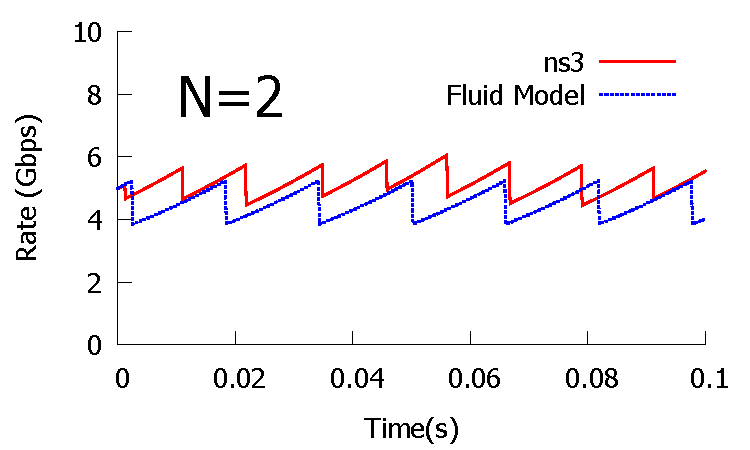
\includegraphics[width=0.3\textwidth]{figures/timely_validation_2_rate.pdf}
}
\subfigure { 
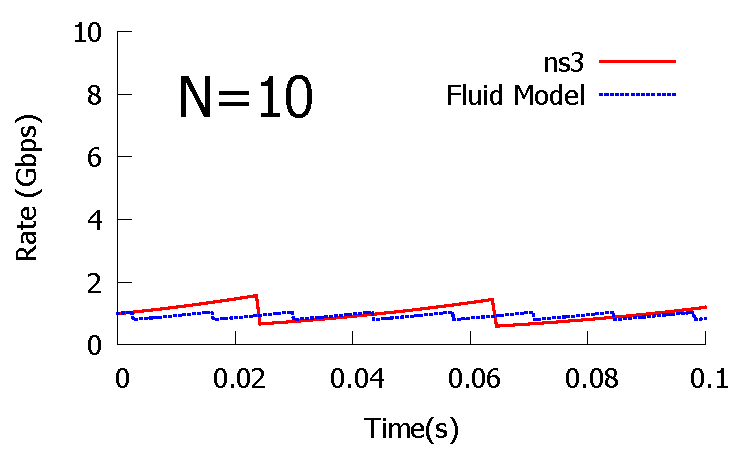
\includegraphics[width=0.3\textwidth]{figures/timely_validation_10_rate.pdf}
}
\subfigure { 
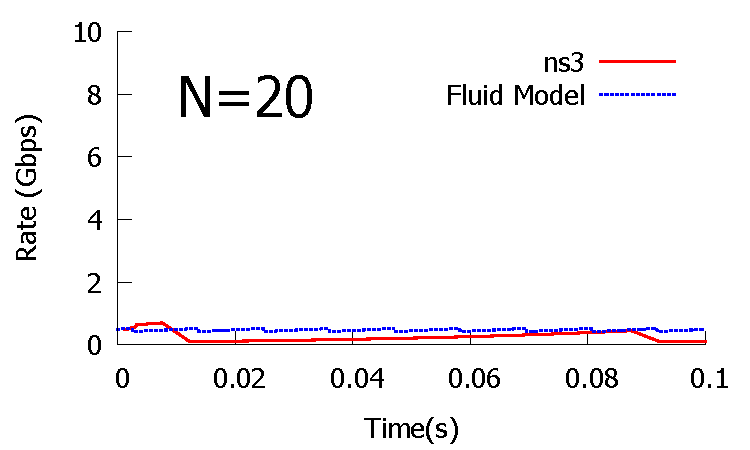
\includegraphics[width=0.3\textwidth]{figures/timely_validation_20_rate.pdf}
}
\vspace{-1em}
\caption{Comparison of TIMELY fluid model and simulations}
\vspace{-1em}
\label{fig:timely_model_validation}
\end{figure*}

